% =========================================================================== %
% TeX input file: "Create the hello world frontend"
%
% WARNING: this tex file does not compile standalone, it needs to be embedded
% in a master tex document (e.g. Introduction.tex)
% =========================================================================== %

The project creation step has created a Scout client that displays an empty desktop form.
We will now add widgets to the client's desktop form that will later display the ''Hello World!'' message.

To add any widgets to the desktop form, we first need to navigate to the \element{DesktopForm} in the Scout Explorer.
For this, first navigate to the orange client node in the Scout Explorer view.
Then, expand the \element{Forms} folder by clicking on the small triangle icon, and further expand the \element{DesktopForm}. 
As a result, the \element{MainBox} element becomes visible below the desktop form as shown in \figref{new_field_context_menu}. 
With a click of the right mouse button over the \element{MainBox}, the available context menus are displayed.
To start the form field wizard we select the \menu{New Form Field ...}.

\begin{figure}
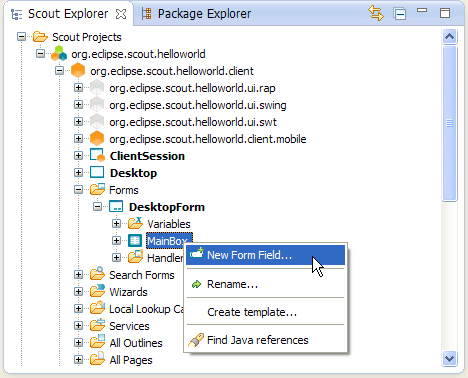
\includegraphics[width=8cm]{sdk_new_field_wizard_menu.png} 
\caption{Using the \menu{New Form Field ...} to start the form field wizard provided by the Scout SDK.}
\figlabel{new_field_context_menu}
\end{figure}

In the first step of the form field wizard shown on in \figref{helloworld_groupboxfield} we choose \java{GroupBox} as the form field type and click on the \button{Next}.
In the second wizard step, we enter 'Desktop' into the \field{Class Name} before we close the wizard with the \button{Finish}.
The Scout SDK will then add the necessary Java code for the \java{DesktopBox} in the background.

\begin{figure}
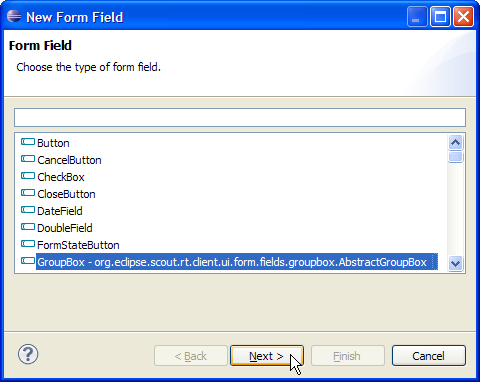
\includegraphics[height=4.5cm]{sdk_new_field_groupbox_1.png} \hspace{8mm}
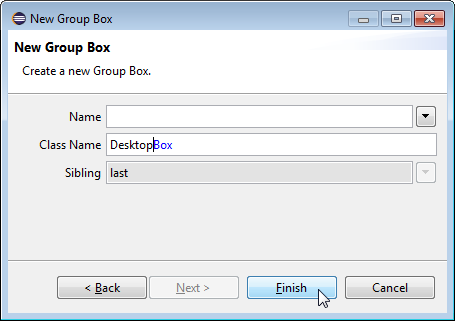
\includegraphics[height=4.5cm]{sdk_new_field_groupbox_2.png}
\caption{Adding the \textit{DesktopBox} field with the Scout SDK form field wizard.}
\index{SDK Wizard!New Form Field}
\figlabel{helloworld_groupboxfield}
\end{figure}

We can now add the text field widget to the group box just created.
To do this, we expand the \element{MainBox} in the Scout Explorer view to access the newly created \element{DesktopBox} element. 
On the \element{DesktopBox} we can then use the \menu{New Form Field ...} again.
In the first wizard step, we select \element{StringField} as the form field type. 
To select the \element{StringField} type you can either scroll down the list of available types or enter ''st'' into the field above the field type list. 

In the second wizard step, we enter 'Message' into the \field{Label}.
As we do not yet have the text 'Message' available in our ''Hello World'' application the wizard prompts the user with the proposal \textsc{New Translated Text ...}.
With a double click on this option a new text entry can be added to the application as shown in \figref{helloworld_stringfield}.
Once we have provided some initial translation for our message label, we can close the translation dialog with the \button{Ok}.
Finally, we close the form field wizard using the \button{Finish}.

\begin{figure}
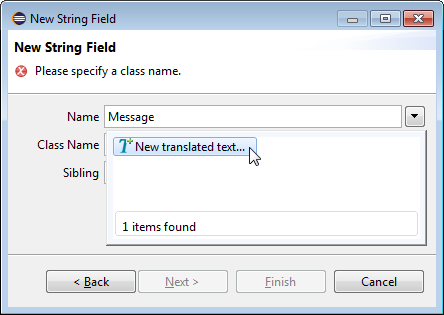
\includegraphics[height=4.2cm]{sdk_new_field_stringfield_1.png} \hspace{8mm}
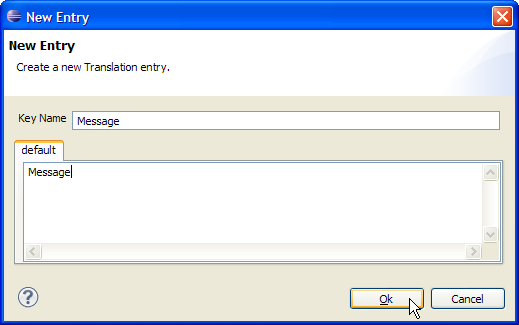
\includegraphics[height=4.2cm]{sdk_new_field_stringfield_2.png}
\caption{Adding a \textit{StringField} and providing a new translation entry.}
\index{SDK Wizard!Add Translation Entry}
\figlabel{helloworld_stringfield}
\end{figure}

By expanding the \element{DesktopBox} element in the Scout Explorer, the new message field becomes visible. 
A double click on the message field element then loads the corresponding Java code into an Editor and displays the message field's properties in the Scout Object Properties as shown in \figref{helloworld_messagefield}.
This is a good moment to compare your status with this screenshot.
Make sure that both the Java code and the project structure in the Scout Explorer look as shown in \figref{helloworld_messagefield}. 

\begin{figure}
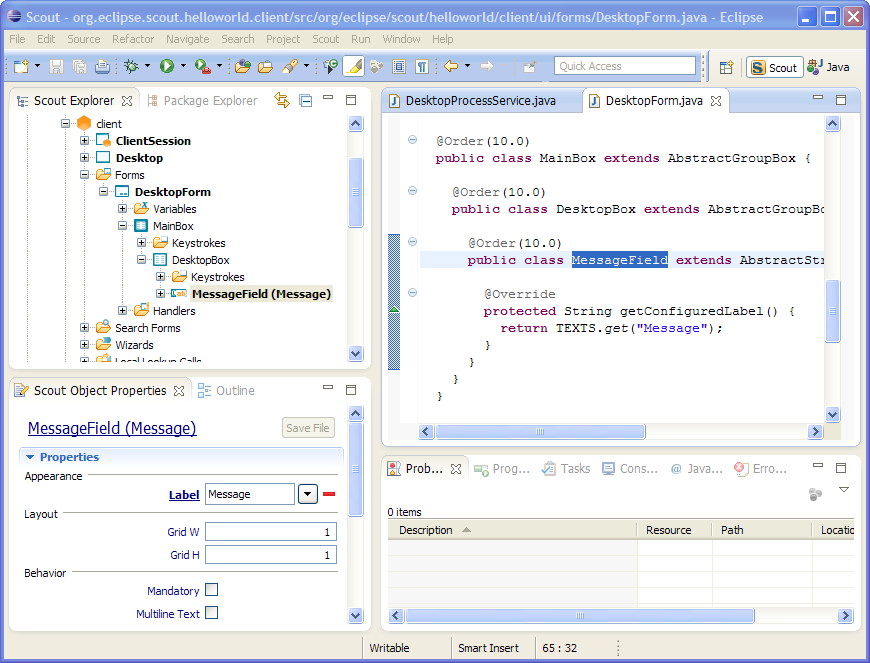
\includegraphics[width=15cm]{sdk_helloworld_messagefield.png}
\caption{Scout SDK showing the \it{MessageField}}
\figlabel{helloworld_messagefield}
\end{figure}

Having verified your status of the ''Hello World'' application you can start the application as described in the previous section.
The client applications will then display your message widget.
However, the text widget is still empty, as we did not yet load any initial content into it.
This is the topic of the next section where we continue this tutorial with the server part.

% =========================================================================== %
% EOF TeX input file
% =========================================================================== %
